\subsection{Case Study}
\label{sec:eval}

We now demonstrate the application of our optimization framework in a case study.  Specifically, we use it to study the placement of a 100MW datacenter and wind farm in the New England transmission network.  Instead of specifying a desired capacity for the wind farm, we assume that we want sufficient wind energy to completely offset the energy consumption of the datacenter (making the size of the wind farm dependent on the weather pattern at its placement location).  This scenario corresponds to when a company wants to build a new datacenter, and a corresponding wind farm to offset the energy use of the datacenter.

\subsubsection{Instantiating the framework parameters}

The production of wind power and datacenter cooling both depend on weather conditions.  Thus, we obtained Typical Meteorological Year (TMY) information for 56 locations in the U.S. New England area as shown in Figure~\ref{fig:NE_locs}.  A TMY is a 1-year dataset of hourly weather values selected to include a representative range of weather phenomena for a location, while still giving annual averages that are consistent with the long-term averages for the location.  The TMY data is obtained from US Department of Energy.\footnote{\url{http://apps1.eere.energy.gov/buildings/energyplus/weatherdata about.cfm}} We use the TMY wind speeds and air pressures, conversion losses, and specifications for the 1.5MW Series wind turbine from General Electric Company \cite{GE15MW} to compute $\beta(l,t)$ at each location $l$ during time epoch $t$.

\begin{figure}[ht]
\centering
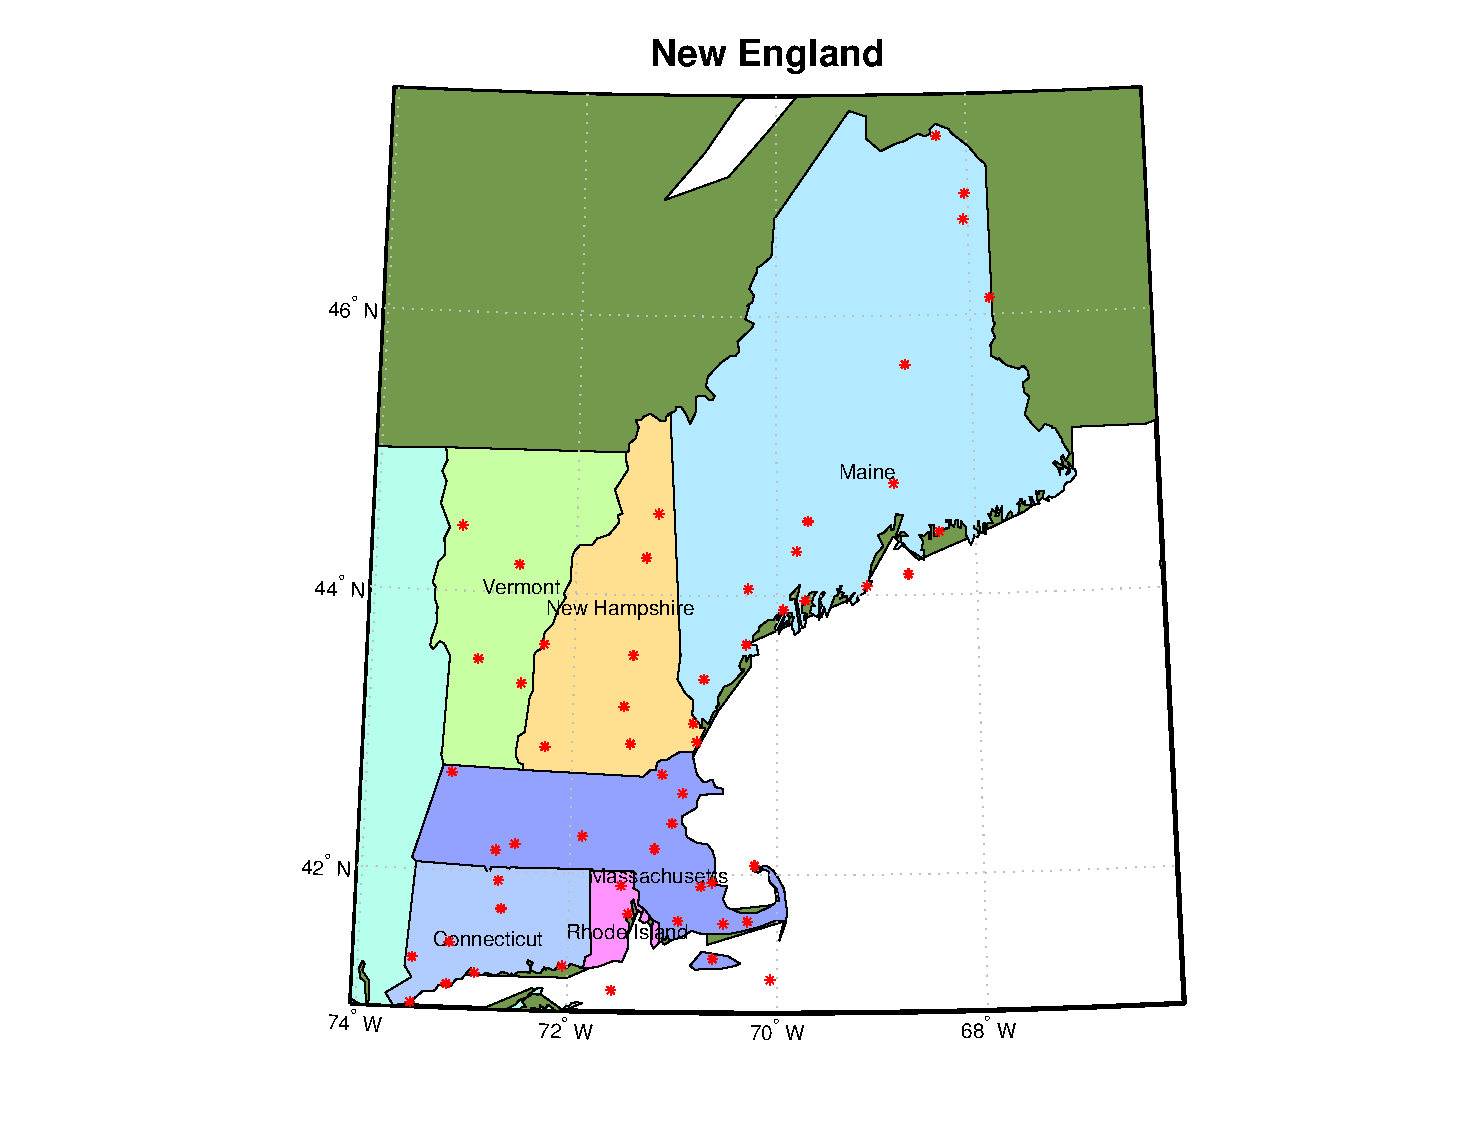
\includegraphics[width=1\columnwidth]{img/NE_map}
\caption{Candidate locations in New England}
\label{fig:NE_locs}
\end{figure}

We adopt the values and approaches for computing PUE, datacenter construction costs, wind farm construction costs, land costs, transmission lines and network connection costs, and grid energy costs from \cite{berral2014building}.  \thunote{I think we need a summary table here to give information.}

\thunote{Xiaoying, what is the assumed load?  What about the datacenter load ($powNeed$)}
For each time epoch $t$, we compute the wind energy being generated by all the wind farms (existing ones and the new one being placed) using $\beta(l,t)$.  We then compute the system loss for the time epoch for the placement of the new datacenter and wind farm at locations $d$ and $w$, respectively, using the simulation approach described in Section~\ref{sec:quantify}.  For each possible pair of ($l$, $w$), we sum the transmission loss over the entire year.

Finally, for the cost of system transmission loss, we set $priceLoss$ to the maximum electricity price in the whole area.  \thunote{Xiaoying, Divya gave us some values that we can use here.  Did we use these new values, or are we still using the maximum electricity price?}

\subsubsection{Placement approach}

To see the impact of considering transmission loss, as well as the simultaneous placement of datacenter and wind farm, we compare results for five different placement approaches:

\begin{itemize}

\item \textbf{DC\_WF\_OPT:} This strategy individually looks for the best location to put the datacenter and the wind farm; i.e., it solves the optimization problem for the datacenter without considering the new wind farm, and then solves the optimization problem again for the wind farm without considering the new datacenter.  This strategy also ignore transmission loss.

\item \textbf{DC+G\_WF+G:} This strategy is the same as DC\_WF\_OPT except that transmission loss is considered when solving the optimization problem.

\item \textbf{Min\_Loss:} This strategy finds locations for the datacenter and wind farm that minimizes the cost of transmission loss.

\item \textbf{Co-location:} This strategy assumes that the datacenter and wind farm 
should be co-located, and so finds a single location for both that minimizes the overall cost.

\item \textbf{Joint:} This strategy considers the simultaneous placement of the datacenter and wind farm, and uses all of the costs and revenues in the optimization framework.

\end{itemize}

\subsubsection{Results}
Figure \ref{fig:cost1dc1wf} shows the results of the total cost by using five different strategies when seeking the best locations when we are building a 100MW datacenter and a wind farm which can supply green energy for it.

From the figure, we can see that by considering grid costs, the total cost will be further saved compared to best choices for the datacenter and the wind farm separately. Also, $Min\_Loss$ can achieve minimal losses of all possible choices, but the total cost is large mainly because it selects an expensive place for purchasing land for the wind farm. The best choice of co-location options is also nearly 7\% higher than the $Jointly$ choice, and it's easy to understand since the best location for datacenter is not necessarily the best for wind farm and vice versa.

We calculate all of the combinations for wind farm and datacenter locations and use the average total cost of these combinations (which is \$667.1M per year) as the baseline for comparison. Then, the locations found and the corresponding cost savings of the five strategies are listed in Table \ref{tab:costsaving}.

\begin{figure}[ht]
\centering
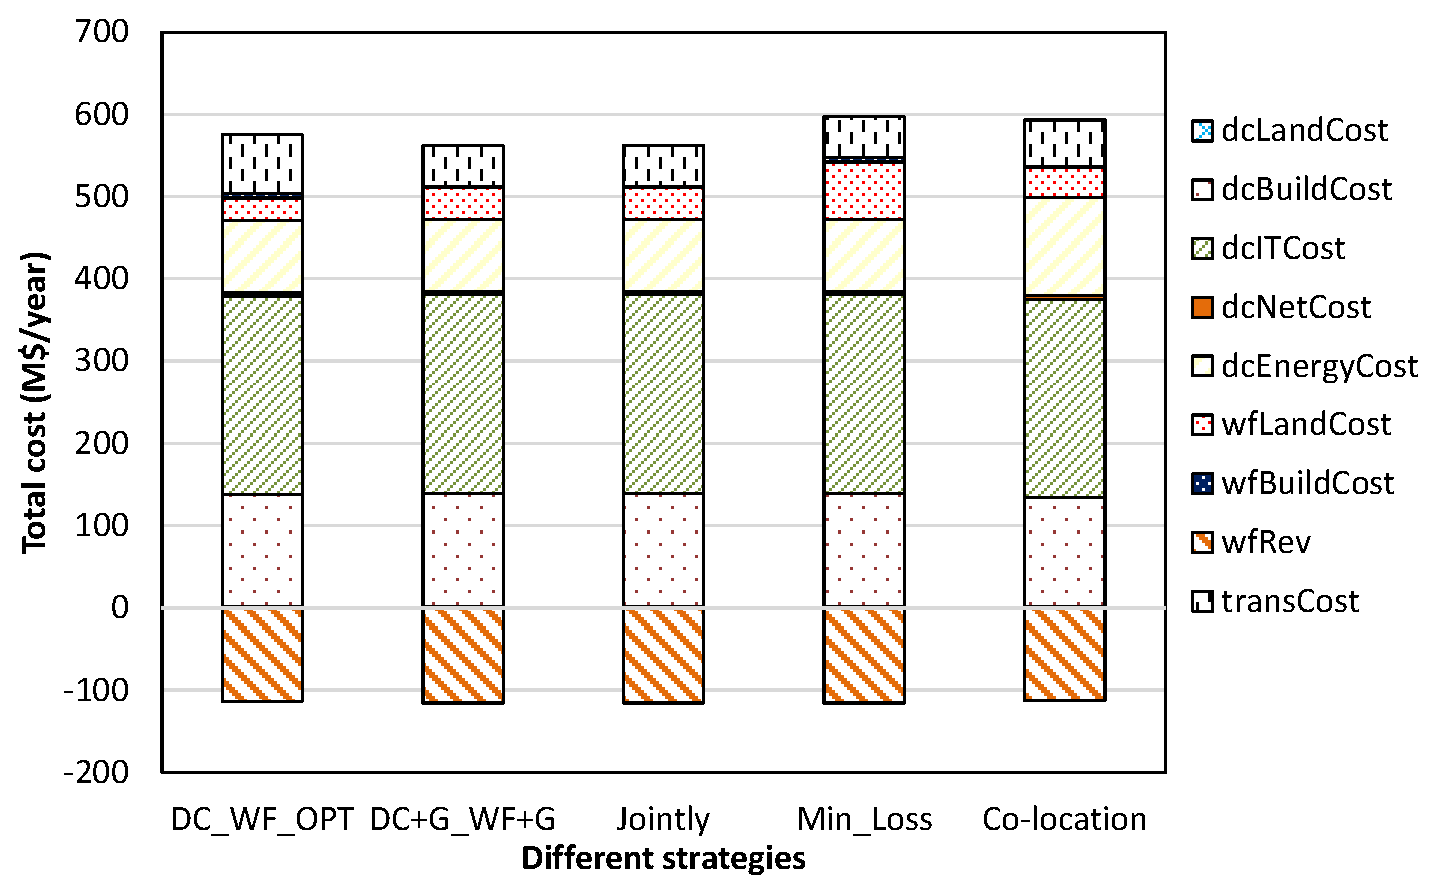
\includegraphics[width=1\columnwidth]{img/cost-one-dc-one-wf}
\caption{Costs of building one datacenter (100MW) with one wind farm}
\label{fig:cost1dc1wf}
\end{figure}

\begin{table}[ht]
\begin{center}
\caption{Detailed results of cost savings by different strategies.}
\begin{tabular}{|l|p{50pt}|p{50pt}|p{30pt}|p{20pt}|}
\hline
\textbf{Strategy}& \textbf{Datacenter location} &\textbf{Wind farm location} &\textbf{Total cost (M\$/year)} &\textbf{Cost saving (\%)} \\
\hline
\textbf{DC\_WF\_OPT} &  Burlington,NH  & Mount Washington, NH &465.6& 30.2 \\
\textbf{DC+G\_WF+G} &Springfield Hartnes, VT  & Nash Island, CO&450.3& 32.5\\
\textbf{Jointly} &Springfield Hartnes, VT&  Nash Island, CO & 450.3 & 32.5\\
\textbf{Min\_Loss} &Springfield Hartnes, VT & Marthas Vineyard, RI & 485.6& 27.2 \\
\textbf{Co-location}& Nash Island, CO &Nash Island, CO&480.7 & 27.9  \\
\hline
\end{tabular}
\label{tab:costsaving}
\end{center}
\end{table}

%%% Local Variables:
%%% mode: latex
%%% TeX-master: "paper"
%%% End:
